% --------------------------------------------------------------------------
% Template for ICAD-2016 paper; to be used with:
%          icad2016.sty  - ICAD 2016 LaTeX style file, and
%          IEEEbtran.bst - IEEE bibliography style file.
%
% --------------------------------------------------------------------------

\documentclass[a4paper,10pt,oneside]{article}
\usepackage{icad2017,amsmath,epsfig,times,url}
\usepackage{hyperref}
\usepackage{hypcap}
\usepackage{cite}

\usepackage{times}
\usepackage[english]{babel}
\usepackage{flushend}

% Example definitions.
% --------------------
\def\defeqn{\stackrel{\triangle}{=}}
\newcommand{\symvec}[1]{{\mbox{\boldmath $#1$}}}
\newcommand{\symmat}[1]{{\mbox{\boldmath $#1$}}}

\newcommand{\ce}[1]{$\mathrm{#1}$}
% Title.
% --------------------
\title{Illustrating trends in nitrogen oxides \\across the United States using sonification}

% *** IMPORTANT ***
% *** PLEASE LEAVE AUTHOR INFORMATION BLANK UNTIL FINAL CAMERA-READY SUBMISSION *** 

% IF ONE AUTHOR , uncomment this part
%\name{Jyri Huopaniemi} 
%\address{Nokia Research Center \\ 
%Speech and Audio Systems Laboratory \\ 
%P.O.Box 407, FIN-00045 Nokia Group, Finland \\ 
%{\tt jyri.huopaniemi@nokia.com}} 
%

% IF TWO AUTHORS, uncomment this part
% \twoauthors{Joshua L. Laughner} {Department of Chemistry \\ University of California, Berkeley \\ Berkeley, CA 94720  USA
% \\ {\tt \href{mailto:jlaughner@berkeley.edu}{jlaughner@berkeley.edu}}} {Elliot Kermit Canfield-Dafilou}
% {Center for Computer Research \\in Music and Acoustics \\ Stanford University,
% Stanford, CA 94305 USA \\ {\tt
% \href{mailto:kermit@ccrma.stanford.edu}{kermit@ccrma.stanford.edu}}}


%%%%%% this was done for anonomization purposes

\twoauthors{} { \\ \\
\\ {\tt \href{}{}}} {}  
{ \\  \\ {\tt  
\href{}{}}}  

%% if necessary, we will uncomment this to reduce the space the bib takes up..
% \let\OLDthebibliography\thebibliography
% \renewcommand\thebibliography[1]{
%   \OLDthebibliography{#1}
%   \setlength{\parskip}{0pt}
%   \setlength{\itemsep}{0pt plus 0.3ex}
% }

\begin{document}
\ninept
\maketitle

\begin{sloppy}

\begin{abstract}
    Leveraging the human auditory system, sonification can be used as educational tool for non-experts to engage with data in a different mode than visualization.  Without oversimplifying the data, this project presents a sonification tool for exploring \ce{NO_2} and \ce{O_3} data from the BErkeley High Resolution (BEHR) Ozone Monitoring Instrument (OMI) and OMO3PR ozone profile datasets.  By allowing the listener control over the data-to-sound mapping and synthesis parameters, one can experience and learn about the interplay between \ce{NO_2} and \ce{O_3} concentrations.  Furthermore, interannual and seasonal trends can be perceived across different types of locations. 
\end{abstract}

\section{Introduction}
\label{sec:intro}

\subsection{Nitrogen oxides play a key role in controlling air quality.}
\label{sec:nox-chemistry}
Nitrogen oxide (\ce{NO}) and nitrogen dioxide (\ce{NO_2}), collectively known as \ce{NO_x}, play an important role in air quality.  Photolysis of \ce{NO_2} produces ozone (\ce{O_3}), and the reaction of \ce{NO} with oxidized volatile organic compounds (VOCs) can lead to the formation of fine particulate matter.

Both ozone and particulate matter concentrations in the atmosphere are regulated by the Environmental Protection Agency (EPA) because of the negative health effects associated with exposure to them. Elevated concentrations of both are known to cause respiratory distress, especially in children \cite{romieu96}. Elevated ozone also damages crops, leading to significant economic losses as well as reducing food yields \cite{tai14}.

The role \ce{NO_x} plays in the production of \ce{O_3} is complex, as the production efficiency of \ce{O_3} depends nonlinearly on both the \ce{NO_x} concentration and the concentrations and identities of VOCs present in the atmosphere. At both high and low concentrations of \ce{NO_x}, \ce{O_3} production due to \ce{NO_x} cycling is suppressed, though for different reasons. At intermediate \ce{NO_x} concentrations, ozone production peaks \cite{murphy07}.  Therefore, cities attempting to improve their air quality by reducing \ce{NO_x} concentrations may see an increase in ozone initially, and a decrease only once \ce{NO_x} concentrations have fallen below a critical point. The value of that critical point depends on the mixture of VOCs present in the atmosphere.

\ce{NO_x} is emitted through a number of processes, both anthropogenic and natural. Anthropogenic sources are typically those involving combustion, as the high temperatures break the \ce{N_2} and \ce{O_2} molecules in the atmosphere, allowing them to recombine as \ce{NO} or \ce{NO_2}. Examples of such sources are vehicles, power plants, ships, and aircraft. Natural sources also include high temperature sources, such as biomass burning or lightning, as well as other sources such as soil bacteria \cite{monks-beirle}.

\begin{figure*}
\centering
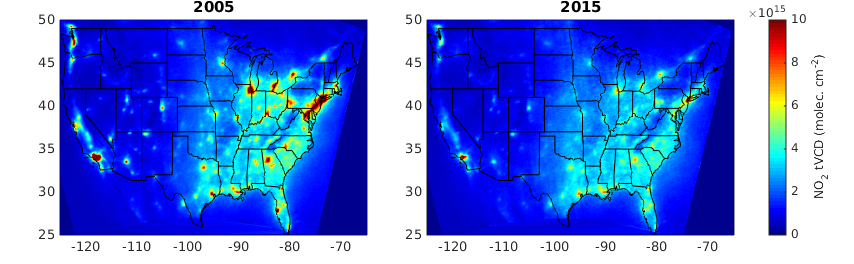
\includegraphics[width=0.9\textwidth]{figs/no2vcds.png} 
\caption{\ce{NO_2} Summertime (Apr--Sept) tVCDs from the BEHR product for 2005 and 2015. A clear decrease throughout the US can be seen.}
\label{fig:sat-obs}
\end{figure*}

\subsection{Space-based measurement of NO$_2$ and O$_3$ offer broad geographic and temporal coverage}

Space-based measurements of \ce{NO_2} tropospheric column density began over two decades ago with the launch of the Global Ozone Monitoring Experiment (GOME) instrument onboard the ERS-2 satellite in 1996 \cite{burrows99}. Only \ce{NO_2}, rather than total \ce{NO_x} is measured due to its spectroscopic properties. Since then, several additional instruments have been launched, including the SCanning Imaging Absorption SpectroMeter for Atmospheric CHartographY (SCIAMACHY) \cite{bovensmann99}, Ozone Monitoring Instrument (OMI) \cite{levelt06}, and GOME-2 \cite{callies00}. All these instruments are carried onboard polar orbiting satellites, allowing them to observe the entire globe in 1--6 days, depending on the instrument and operational mode.

Space-based observations of \ce{NO_2} offer a level of combined spatial and temporal coverage not possible with ground- or aircraft- based instruments.  This offers several notable advantages, such as the ability to observe an entire urban and suburban area, to compare multiple urban areas across the globe using the same instrument, as well as the ability to monitor episodic events (biomass burning, lightning) difficult to track with other types of instruments.  Multiple papers have made use of these properties to investigate both anthropogenic \cite{ding15, lamsal15, tong15, huang14, vinken14, gu13, miyazaki12, russell12, lin10, kim09} and natural \ce{NO_x} emissions \cite{miyazaki14, beirle10, castellanos14, mebust14, mebust13, zorner16}.

The result of these measurements is a ``tropospheric vertical column density'' (tVCD), usually in units of molecules/cm$^2$. This is the total number of molecules of \ce{NO_2} over one square centimeter of the Earth's surface between the surface and the top of the troposphere (typically $\sim$ 12 km). Rural areas considered ``clean'' typically have tVCDs of $\leq 1 \times 10^{15}$ molec. cm$^{-2}$. Highly polluted areas such as Los Angeles, CA, USA or Beijing, China have tVCDs in excess of $1 \times 10^{16}$ molec. cm$^{-2}$.

Measurements of \ce{O_3} from space can be done similarly to measurements of \ce{NO_2} using ultraviolet-visible spectroscopy and are almost always measured by the same satellites. However, measurements of \emph{tropospheric} \ce{O_3} are complicated by the high concentration of \ce{O_3} in the stratosphere. Whereas the tropospheric and stratospheric components of the total \ce{NO_2} vertical column density are similar orders of magnitude, the tropospheric component of the \ce{O_3} total VCD is minor compared to the stratospheric component \cite{monks-beirle}. Alternatively, the retrieval of tropospheric \ce{O_3} may be done using infrared spectroscopy \cite{nassar08}.

\subsection{NO$_x$ has decreased in the US over the past decade.}
\label{sec:nox-decrease}

In the US, the Environmental Protection Agency (EPA) has regulated measures to decrease the emissions of \ce{NO_x} in order to reduce tropospheric ozone concentrations \cite{epa99}. Regulations targeted both vehicular emissions \cite{epa16} and power plant emissions \cite{epa-cair}.  Satellite observations of \ce{NO_2} \cite{russell12, kim09, lu15} can clearly see the decrease in \ce{NO_2} throughout the US for the time period 2004 onwards (Fig. \ref{fig:sat-obs}).

\subsection{Sonifcation is an ideal educational tool to communicate the complexity of NO$_x$/O$_3$ chemistry.}

\begin{figure}
\centering
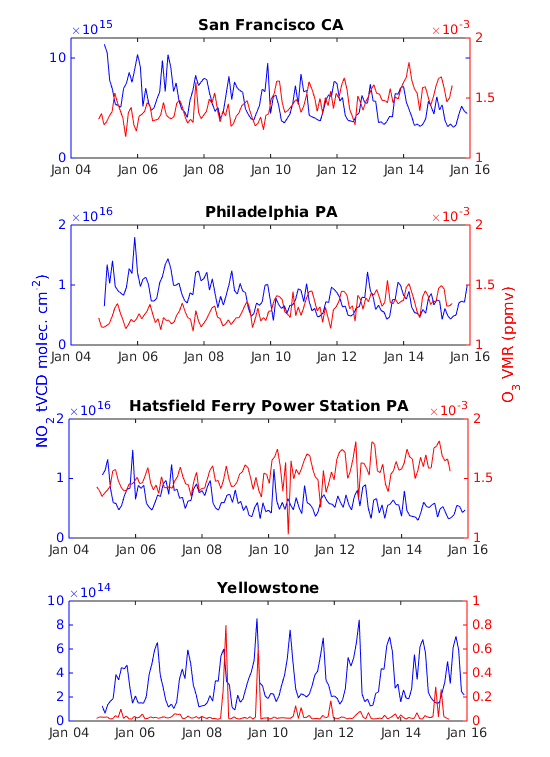
\includegraphics[width=0.5\textwidth]{figs/four-site-trends.png} [htb]
\caption{\ce{NO_2} tVCD and \ce{O_3} surface concentration trends at two cities (San Francisco, CA and Philadelphia, PA), one coal-fired power plant (Hatsfield, in Masontown, PA) and Yellowstone National Park (WY).}
\label{fig:trends}
\end{figure}

\ce{NO_x} and \ce{O_3} have interesting temporal patterns on both the interannual and seasonal time scales. As discussed in \S\ref{sec:nox-decrease}, \ce{NO_x} has, in general, decreased across the US in the past decade. \ce{NO_x} concentrations also follow a seasonal cycle, owing to temperature dependent shifts in the chemistry, leading to a sinusoidal pattern superimposed on top of the interannual decrease.  The chemistry described in \S\ref{sec:nox-chemistry} means that \ce{O_3} concentrations will be related to \ce{NO_x} concentrations, but the exact dependence will vary from location to location.

This is shown in Fig. \ref{fig:trends} for two cities, one power plant, and one rural area. Both seasonal and interannual trends are clear. The cities and power plants exhibit maximum \ce{NO_2} values in the winter, while the rural location does so in the summer. Overall, \ce{NO_2} tVCDs decrease over the cities and power plant, while remaining fairly constant over Yellowstone. \ce{O_3} appears to increase over the interannual time scale for the cities and power plant, but not over Yellowstone. 

These characteristics make sonification an ideal way to describe the \ce{NO_x}/\ce{O_3} relationship throughout the US. The temporal dependence of the data lends itself naturally to depiction in a time-dependent medium such as sound. The geographically diverse natural of the dataset can be well represented by the placement of sound in the panning field. By simultaneously representing the \ce{NO_2} and \ce{O_3} concentrations at multiple cities, power plants, and rural areas across the US, we provide an intuitive interface for the public to learn about how reductions in \ce{NO_x} concentrations affect \ce{O_3} under different conditions.
	
\begin{figure}[t]
\centering
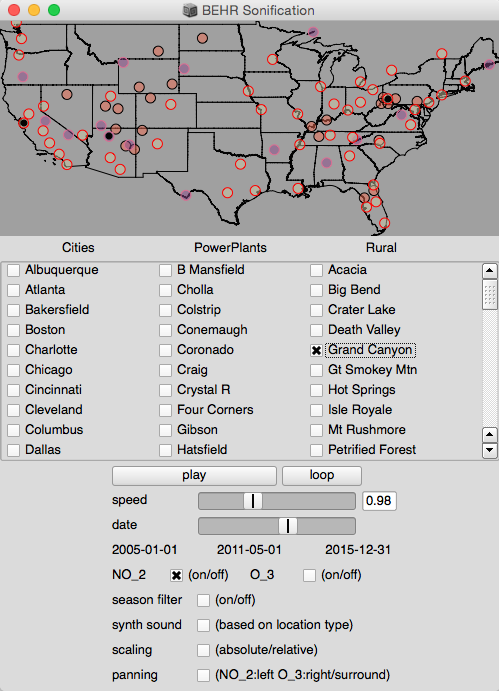
\includegraphics[width=0.5\textwidth]{figs/gui.png}
\caption{BEHR Sonification GUI.}
\label{fig:gui}
\end{figure}

\section{Approach to sonification}
As an educational tool, sonification allows the user to engage with data in a completely different mode than visualization. The streaming capabilities of the human auditory system makes it good at processing multiple, synchronous data series. As \S \ref{sec:nox-chemistry} describes, the interactions of atmospheric chemicals, meteorological conditions, and ground activity are extremely complicated. Nevertheless, at various time scales, the trends in \ce{NO_2} and \ce{O_3} can be intuitively understood through the auditory experience. Unlike data-music, this sonification project has distinct educational goals and is designed for non-experts in particular. While we strive to reduce the complexity of the data, we want the sonification model to convey useful information.  Furthermore, we want an interface that gives the user flexibility to determine how the data should be presented.  This fulfills the goal to let the user explore the data in a way that conveys pertinent information.  

\subsection{NO$_2$ satellite dataset}
	We make use of v2-1C of the BErkeley High Resolution (BEHR) Ozone Monitoring Instrument (OMI) \ce{NO_2} gridded product, which is publicly available at \url{http://behr.cchem.berkeley.edu/DownloadBEHRData.aspx}. The BEHR dataset is chosen because it uses high-resolution \emph{a priori} \ce{NO_2} profiles that better resolve the urban/rural \ce{NO_2} gradient than the NASA Standard Product or the KNMI DOMINO product. The OMI is carried on board the NASA Aura satellite, launched in 2004, and is a nadir-viewing, UV-visible spectrometer with an overpass time of 13:30--14:00 local standard time \cite{levelt06}.
	
	We use the cities and power plants identified in Russell et al. 2012 \cite{russell12} as the sites for urban and power plant trends. We choose 15 additional sites in rural areas, focusing mostly on national parks, to demonstrate \ce{NO_2} variability in areas substantially less influenced by anthropogenic emissions. The radii for these sites are set to 40 km; this choice is arbitrary, as there is no clear plume to encompass, but is similar to the average radius used for the cities. Monthly average \ce{NO_2} tropospheric vertical column densities (tVCDs) are used to generate the trends. First, the gridded product is restricted to data meeting the following criteria:
	
	\begin{itemize}
	\item Cloud fraction $\leq 0.2$
	\item The XTrackQualityFlags value must be 0 for all pixels that contribute to this grid cell
	\item The vcdQualityFlags must be an even integer (least significant bit is 0)
	\item Only rows 1--58 (0 based indexing) are used due to an issue in v2-1C of the BEHR product that causes the edge rows to be too large.
	% This is NOT the row anomaly; the row anomaly is something very specific with all OMI products
	\end{itemize}
	
	The gridded data is temporally averaged, weighted by the inverse of the pixel areas that contribute to the grid cells. This gives more weight to smaller, more representative pixels.  For each monthly average, the grid cells whose centers are within the radius of the site longitude and latitude given in \cite{russell12} are then themselves averaged to give a single value for each site for each month.

\subsection{O$_3$ satellite dataset}

	We use the OMO3PR ozone profile dataset to obtain tropospheric \ce{O_3} available from \url{https://disc.gsfc.nasa.gov/Aura/data-holdings/OMI/omo3pr_v003.shtml}.   This retrieval uses optimal estimation to fit an \ce{O_3} profile to observed absorbance in two wavelengths. An \emph{a priori} \ce{O_3} profile is used as the basis for the profile shape.  We choose this product because it is also derived from the Ozone Monitoring Instrument, as is our \ce{NO_2} product, and so has similar spatial and temporal coverage. Kroon et al. compared this product again multiple other satellite \ce{O_3} products and \emph{in situ} sonde measurements and found a +30\% bias in the midlatitudes  \cite{kroon11}. While this alone should not interfere significantly in the use of this product for the trend sonification in this work as the bias is systematic, uncertainty in the values may still be high due to the challenge of separating tropospheric and stratospheric \ce{O_3}.
	
	A gridded version of this product is not available; therefore we obtain monthly averages differently than with the \ce{NO_2} product. Similarly to \ce{NO_2}, pixels with centers within the radii defined for the geographic sites are identified as contributing to the trend for that site; unlike the \ce{NO_2} product, these are the native satellite pixels, rather than regridded data. All valid pixels for a site for a month are binned in this step. Pixels are considered invalid if:
	
	\begin{itemize}
	\item Cloud fraction for either UV channel is $> 0.2$
	\item Aerosol optical thickness is $> 10^{-5}$. Elevated aerosol layers lead to erroneously large tropospheric \ce{O_3} concentrations \cite{omo3pr-readme}.
	\item The ReflectanceCostFunction field is $> 30$. This indicates erroneous radiance due to the OMI Row Anomaly \cite{row-anomaly}.
	\end{itemize}
	
	For each binned profile, two quantities are calculated. First, the bottom partial column (in Dobson Units) is converted into volume mixing ratio in units of part-per-million by volume (ppmv) using the formula provided in the OMO3PR Readme \cite{omo3pr-readme}. Because this formula relies on the edges of the pressure bin and the lower edge is the surface, we calculate the surface pressure for each profile by interpolating the Global Lane One-km Base Elevation (GLOBE) project elevation data \cite{globe} to the pixel latitude and longitude, then convert from altitude to pressure using Eq. \eqref{eqn:pres-scale-height}:
	
	\begin{equation}
	\label{eqn:pres-scale-height}
	p = p_0 e^{-z/H}
	\end{equation}
	
	where $p_0$ is the sea level pressure of 1013 hPa, $z$ is the altitude in meters, and $H$ is a scale height of 7400 m.
	
	The second quantity is the tropospheric vertical column density (tVCD), which is computed by summing the profile partial columns over all levels with a bottom pressure edge $> 200$ hPa. This is converted from Dobson Units to molec. cm$^{-2}$ by multiplying by $2.69 \times 10^{16}$
molec. cm$^{-2}$ / DU. 

	Both the surface concentration and tVCD are averaged over all pixels binned to a given site for a given month. Unlike the \ce{NO_2} product, no weighting for pixel area is applied, as the pixel size is not given in this product.
	 
\subsection{Sonic Mappings}
\label{sec:sonic-mappings}
After the preprocessing, we have a set of locations through the United States that each have corresponding time series for \ce{NO_2} and \ce{O_3}. We present several modes for listening to the data. In the simplest case, we use the data for each location as the frequency parameter to a simple sinusoidal oscillator.  We exponentially map all the values of the compounds' into an audible range such that 
\begin{align}
    \text{min}_{\text{global}}(\text{\ce{NO_2}}) &\rightarrow
    \text{min}(\text{freq}_1) \\
    \text{max}_{\text{global}}(\text{\ce{NO_2}}) &\rightarrow
    \text{max}(\text{freq}_1) \\
    \text{min}_{\text{global}}(\text{\ce{O_3}}) &\rightarrow
    \text{min}(\text{freq}_2) \\
    \text{max}_{\text{global}}(\text{\ce{O_3}}) &\rightarrow
    \text{max}(\text{freq}_2)
    \,,
\end{align}
and the mapping is
\begin{equation}
    c \left[(c/d)^{\frac{x-a}{b-a}}\right]\,,
\end{equation}
where $x$ is the value being mapped from the old range $[a, b]$ to the new range $[c, d]$.  Thus, \ce{NO_2} and \ce{O_3} can be constrained to different frequency ranges, scaled according to their independent global minimum and maximum values.  The chemical compounds are presented in their own audio channels so they can be more easily differentiated.  One can choose to listen to one or more location, and since the ranges are scaled by a common mapping, the data are sonically comparable. This model is compelling as individual geographical locations can be easily compared to one another. However, as the number of geographical locations increases, it becomes challenging to track specific locations. 

To address this issue, we propose using band-pass filtered triangle waves for each geographical location and the incorporation of panning. By placing the listener at the center of the United states, we can calculate the angle at which each location should appear, given the direction the listener is facing.  For this, we use an eight channel speaker system that inscribes the listener, and we map the cities to the correct location using equal-power panning between neighbor-pairs of speakers.  The more complex waveform is required to improve localization cues.  

In order to bring out some features of the data we provide several more options. First, we can highlight seasonal fluctuations by controlling the $Q$ factor of the band-pass filter as a function of season. This highlights the effects of annual seasonal changes. Second, we provide the ability to change the waveforms used in the sonification of location types. While it is useful to compare \ce{NO_2} and \ce{O_3} concentrations, this feature allows power plant, cities, and rural areas to stand out from one another. Additionally, while it is useful to compare locations, some have a smaller extent than others. To address this, we also provide the ability to scale the data for each location by its own minimum and maximum rather than the global \ce{NO_2}/\ce{O_3} minimum and maximum.  


\subsection{Sonification interface}

While the synthesis routines do not depend on the GUI, having an interface makes it much easier to understand and control what one listens to. The GUI, which can be seen in Fig. \ref{fig:gui}, displays a map of the United State with indicators for where we present data.  These locations are color coded by location type (e.g., power plants, cities, etc.). A bank of check-boxes allow the user to select which locations contribute to the sonification. Naturally, the map is updated to reflect which locations are selected.  


Basic control is provided for playing/pausing and loudness. We also provide the ability to loop through the data or stop once the listener reaches the most current month.  Controls are also provided to control the speed at which the sonification is performed.  When the data are presented quickly, the listener perceives general trends while at slower speeds the seasonal and monthly trends dominate.  This time resolution control is useful for zooming between micro and macro scales.  

Finally, controls are offered for switching between the various sonification schemes. We provide the appropriate controls to enable/disable features of the model, and when appropriate, control their parameters.  

\subsection{Evaluation}

\subsubsection{NO$_2$ interannual trends}
The \ce{NO_2} trends are quite apparent both for a single location and when comparing multiple locations.  When using the global scaling, the seasonal oscillation in \ce{NO_2} concentrations stands out quite clearly, especially for cities. For rural environments, the global scaling compresses the values.  This is useful, however, for comparing them to urban locations.  Aurally, it is obvious that the overall \ce{NO_2} levels are much lower in rural environments. Using the local scaling, the downward trends and seasonal oscillatory trends become more apparent. 

In general, power plants seem to be less effected by seasonal changes than cities, but listening to the locally scaled version of the power plants makes the season changes more apparent. One interesting observation is that some power plants (e.g., Huntington) start with a sharp decrease in \ce{NO_2} emissions which then level out for the rest of the dataset. Overall, these observations provide compelling evidence for the importance of both scaling options.  

Another interesting observation is that locations on the East Coast tend to have higher overall levels than elsewhere in the country.  For example, Shenandoah is in rural Virginia, however the \ce{NO_2} levels are comparable to those in Fresno, California.  Naturally, Shenandoah's  \ce{NO_2} levels are influence by its proximity to large cities like Baltimore. Likewise, trends in Philadelphia and Pittsburgh are very correlated to one another. 

\subsubsection{O$_3$ interannual trends}
For evaluation, we use the \ce{O_3} concentration nearest the surface rather than the partial \ce{O_3} column.  Informal listening tests show that patterns are apparent even to listeners without extensive knowledge of \ce{NO_x}/\ce{O_3} trends and chemistry.  An overall rise observed in most cities is readily apparent, as are the seasonal oscillations. 

This also indicates that the OMO3PR product shows \ce{O_3} is increasing on the interannual timescale throughout the US. This is consistent with the hypothesis that \ce{O_3} increases with temperature \cite{lin17}. However, due to the difficulty in retrieving tropospheric \ce{O_3} from space, verifying this with other tropospheric \ce{O_3} satellite products (e.g. \cite{choi08}) should be considered, and comparison to surface-based measurements should be carried out. Additionally, we are planning on including temperature data to demonstrate the relationship between \ce{O_3} and temperature.  Nevertheless, the listener can clearly hear interannual trends in the \ce{O_3} retrieved with the OMO3PR product; thus the sonification itself represents this successfully and can be used with other \ce{O_3} measurements in the future.

\ce{O_3} faces some challenges, given that the data has more extreme values compared to \ce{NO_2}. These are comparatively infrequent, but significantly larger than the majority of values.  In our current mapping, this means that the majority of the variability is compressed to a very small range. This can be alleviated by doing the same mapping as described in \S\ref{sec:sonic-mappings}, but by clipping the range to prevent outliers from having such an effect on the rest of the data.  This will make the interannual variability much clearer for most sites, but means the listener cannot compare absolute magnitudes. 
% Additionally, at sites with the infrequent, extreme values (e.g. Los Angeles), hearing the interannual trend even in this ``local'' mode is difficult.
 

\subsubsection{Relationship between NO$_2$ and O$_3$}

	As described in \S\ref{sec:nox-chemistry}, the changes in \ce{O_3} concentration can be positively or negatively correlated with changes in the \ce{NO_x} concentrations. Identifying this correlation sonically is challenging, but this is in part because the correlation is weak itself. To examine this, we listened to the \ce{NO_2} and \ce{O_3} trends for Phoenix, AZ\footnote{A city not previously examined graphically} with \ce{NO_2} and \ce{O_3} in distinct channels, and the speed slowed down to $\sim 2$ data points per second.  Although the task was difficult, a listener trained in \ce{NO_x}/\ce{O_3} chemistry could identify times when positive and negative correlations exist.  
	
	\begin{figure}
	\centering
	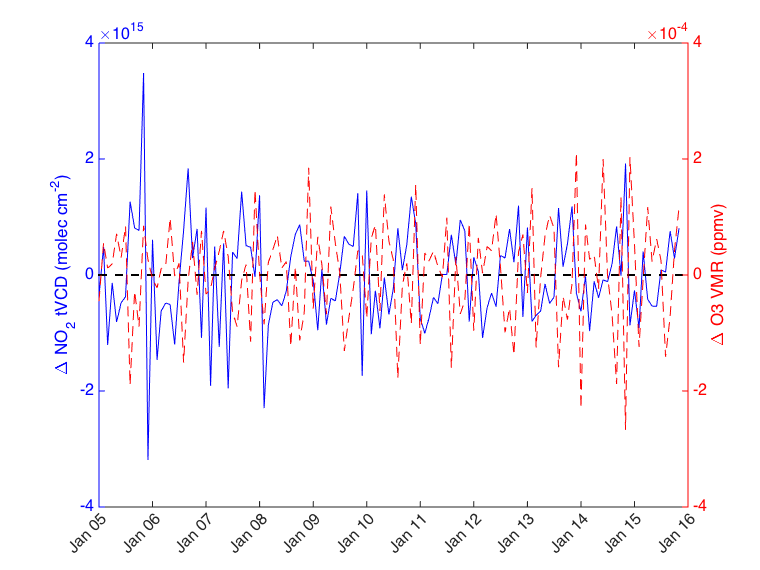
\includegraphics[width=0.5\textwidth]{figs/delta-delta-timeser-phoenix_AZ.png} 
	\caption{Delta-delta time-series plot of \ce{O_3} and \ce{NO_2} for Phoenix, AZ.}
	\label{fig:del-del}
	\end{figure}
	
	Fig. \ref{fig:del-del} plots the change in  between adjacent data-points as a function of time for Phoenix, AZ. The overall correlation between \ce{NO_2} and \ce{O_3} is negative, although there are times when the correlation is positive, as was deduced from listening. While both the graphical and sonic representation of this relationship are challenging, we believe that the sonic representation is ultimately more significantly more engaging for a non-expert.

\section{Conclusions}
In this paper, we have described a sonification tool for comparing trends in \ce{NO_2} and \ce{O_3} concentrations across the United States.  Overall, informal listening tests have shown that untrained listeners can  hear trends across multiple time scales and differences between various locations for which we provide data.  Clearly, there is more work to be done. We need to provide additional data such as temperature and humidity as well as ground based measurements to improve the educational value of presenting the data as a sonification for untrained listeners.  Furthermore, while this project focuses on an experiential auditory experience for non-experts, we should provide more visual feedback (e.g., generating plots on-the-fly that correspond to the sonification) as an additional avenue for learning about \ce{NO_2} and \ce{O_3} trends.  


\section{ACKNOWLEDGMENT}
\label{sec:ack}

JLL acknowledges support from NASA through the Earth and Space Science Fellowship NNX14AK89H, NASA grants NNX15AE37G and NNX14AH04G, and the TEMPO project grant SV3-83019.  JLL also thanks Ronald C. Cohen for advice and support as a Ph.D. advisor.


% -------------------------------------------------------------------------
% create the bibliography
\bibliographystyle{IEEEtran}
% \footnotesize{
\bibliography{refs2014}
% }


\end{sloppy}
\end{document}
